
\section{Results}
\label{sec:results}

\begin{figure*}[t]
\begin{subfigure}{\textwidth}
    \centering
    \begin{subfigure}[t]{0.5\textwidth}
        \centering
        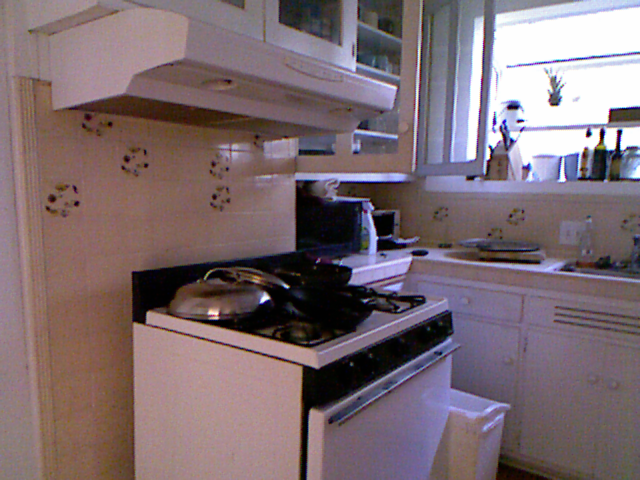
\includegraphics[height=.7\textwidth]{figs/Original321.png}
        \caption{Color}
        \label{fig:original:color}
    \end{subfigure}%
    ~ 
    \begin{subfigure}[t]{0.5\textwidth}
        \centering
        
\includegraphics[height=.7\textwidth]{figs/Depth321.png}
        \caption{Depth (in greyscale)}
        \label{fig:original:depth}
    \end{subfigure}
\end{subfigure}

\vspace{.1in}

\begin{subfigure}{\textwidth}
    \centering
    \begin{subfigure}[t]{0.5\textwidth}
        \centering
        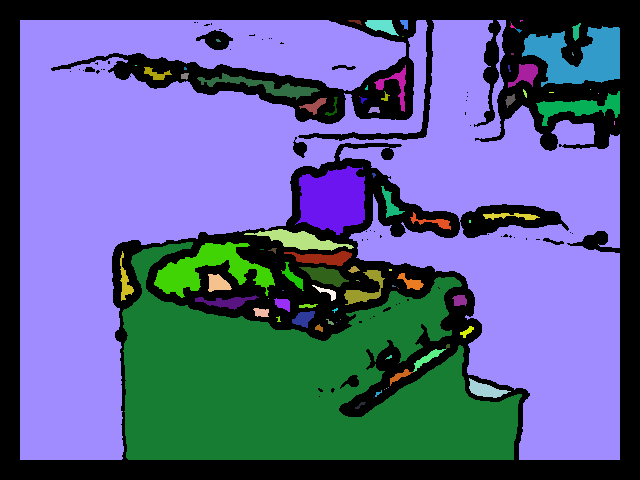
\includegraphics[height=.7\textwidth]{figs/Laplacian321.png}
        \caption{Laplacian Edge Detection}
        \label{fig:results:laplacian}
    \end{subfigure}%
    ~ 
    \begin{subfigure}[t]{0.5\textwidth}
        \centering
        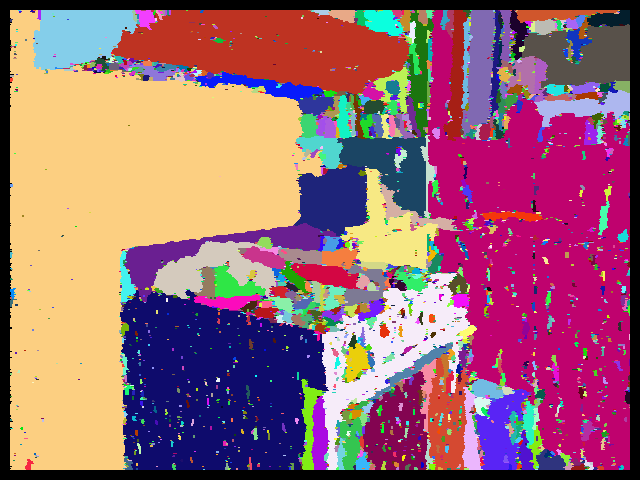
\includegraphics[height=.7\textwidth]{figs/Gradient321.png}
        \caption{Gradient Surface Detection}
        \label{fig:results:gradient}
    \end{subfigure}
\end{subfigure}
\caption{The segmentation of a kitchen scene featuring a stove, oven hood, and cabinets using the Laplacian and Gradient algorithms \cite{kinect}.}
\end{figure*}

The fundamental difference in the detection techniques between the algorithms has a highly noticeable effect.  Because LED is sensitive to jump discontinuities, edges of objects and surfaces go unnoticed if they coincide with the edge of another surface, such as on corners.  This effect is visible in  Fig.~\ref{fig:results:laplacian}, where the stove in the center of the image has been correctly segmented, but the front-facing corner of the stove is not reflected in the segmented image.  The jump discontinuities at the back edges of the stove separate it from the wall and cabinets sufficiently to register as a distinct object.

GSD, on the other hand, reliably detects corners and surface edges.  The faces of the stove are clearly visible in Fig.~\ref{fig:results:gradient}, and sufficient difference in normal vector exists between the wall and the edges of the stove to separate the two into separate regions, like in Fig.~\ref{fig:results:laplacian}.  

It is important to note that reliable behavior for these algorithms was hard to find.  Different images required tuning to see meaningful results, as a correctly chosen blur radius and edge threshold are crucial to detecting meaningful edges in LED and angle threshold defines GSD's ability to group regions.  Segmenting an image containing slat-style window blinds with LED, for example, requires a relatively large blur radius and threshold to avoid segmenting every individual slat in the blinds.  Alternatively, if that behavior is desired, the radius and threshold can be lowered.  These changes, though, also alter the algorithm's ability to correctly distinguish other objects within the image, with large radii and thresholds blurring objects out of existence and small values incorrectly grouping small bumps or, as discussed below, flaws in the image.

In general, the GSD algorithm required a cleaning algorithm to partially handle the speckling problem visible in Fig.~\ref{fig:results:gradient}.  We believe this behavior occurs due to random flaws in image quality -- the result of using a realistic data set.  LED is fairly robust to these fluctuations because of the averaging effect of the blur, but because GSD calculates the normal vector for every pixel, it is sensitive to small errors in the data.  While a small Gaussian blur would have likely removed most of the flaws, the blur also averages data around corners, rendering the normal vectors less accurate and essentially decreasing the resolution of the depth image.  Because GSD is sensitive to small differences in surfaces, it is less reliable on images with small details, such as the slat-style window blinds mentioned above, which were frequently grouped into arbitrary, inconsistent regions.